\documentclass[border=10pt]{standalone}

\usepackage{tikz}
\usepackage{tikzsymbols}
\usetikzlibrary{calc,patterns,shapes.geometric}

\def\centerarc[#1](#2)(#3:#4:#5){\draw[#1] ($(#2)+({#5*cos(#3)},{#5*sin(#3)})$) arc (#3:#4:#5);}

\begin{document}
	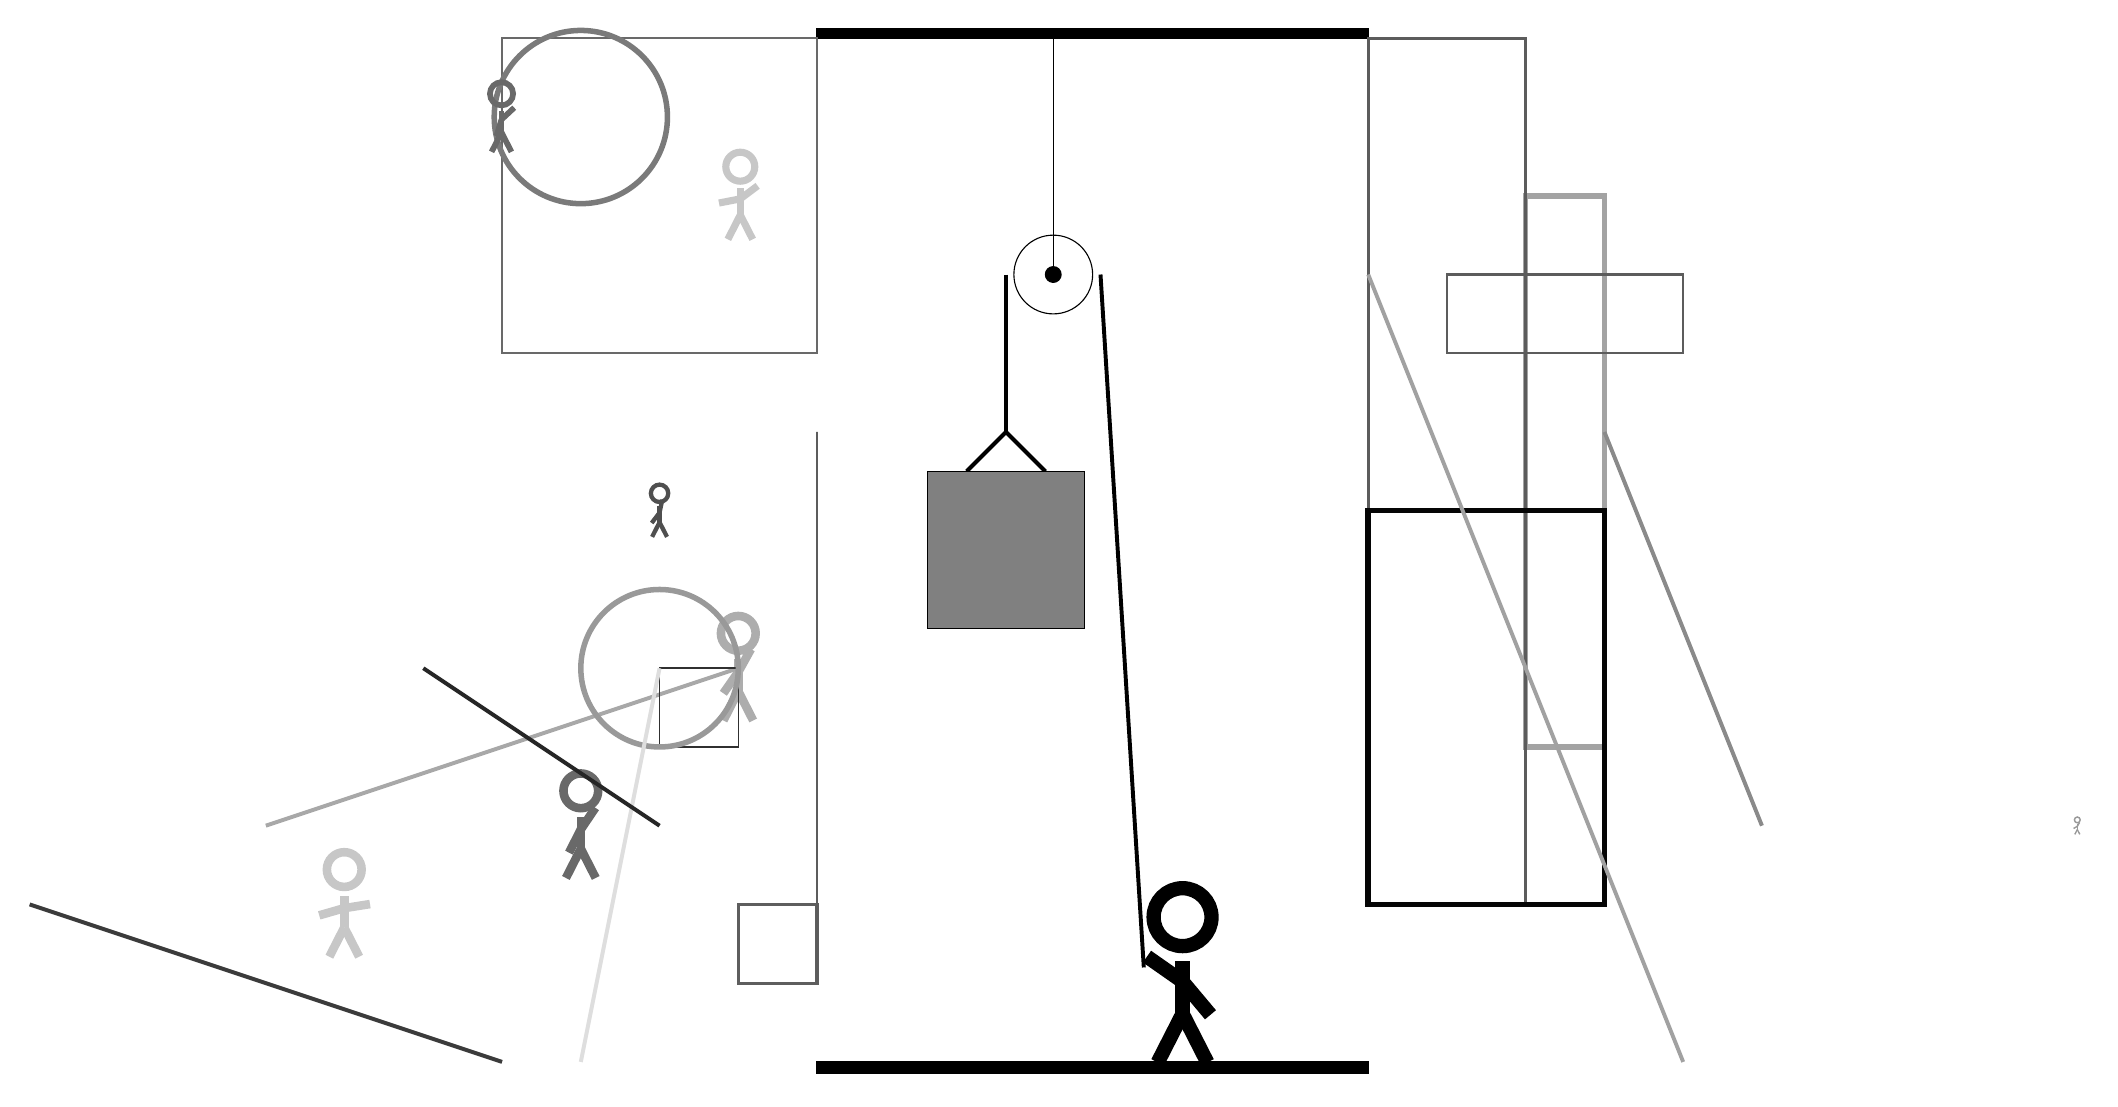
\begin{tikzpicture}
		%%%%% START %%%%%
		
		\draw[fill=black] (-2, 10) rectangle (5, 10.125);
		
		\draw[line width=0.3mm, color=black!59] (-2, 6) rectangle (-6, 10);
		
		\draw[line width=0.7mm, color=black!36] (7, 1) rectangle (8, 8);
		\draw[line width=0.4mm, color=black!64] (7, 10) rectangle (5, -1);
		\draw[line width=0.3mm, color=black!64] (6, 7) rectangle (9, 6);
		\node[line width=0.5mm, color=black!59] at (-5, 0) {\Strichmaxerl[6][63][56]};
		\draw [line width=0.7mm, color=black!52](-5, 9) circle (1.1);
		\draw[line width=0.7mm, color=black!98] (5, 4) rectangle (8, -1);
		\draw[line width=0.4mm, color=black!63] (-2, -2) rectangle (-3, -1);
		\node[line width=0.3mm, color=black!32] at (-3, 2) {\Strichmaxerl[6][55][61]};
		
		\draw[line width=0.5mm, color=black!34](-3, 2) -- (-9, 0);
		
		\node[line width=0.7mm, color=black!59] at (-6, 9) {\Strichmaxerl[4][73][43]};
		\node[line width=0.5mm, color=black!69] at (-4, 4) {\Strichmaxerl[3][53][78]};
		\draw[line width=0.2mm, color=black!81] (-3, 1) rectangle (-4, 2);
		
		\draw[line width=0.3mm, color=black!64] (-2, 5) rectangle (-2, -2);
		\draw[line width=0.5mm, color=black!37](9, -3) -- (5, 7);
		\node[line width=0.6mm, color=black!22] at (-8, -1) {\Strichmaxerl[6][16][9]};
		
		\draw[line width=0.3mm, color=black!11] (-3, 4) rectangle (-3, 4);
		\draw[line width=0.5mm, color=black!46](10, 0) -- (8, 5);
		\draw[line width=0.5mm, color=black!77](-6, -3) -- (-12, -1);
		
		\node[line width=0.4mm, color=black!22] at (-3, 8) {\Strichmaxerl[5][11][37]};
		\draw [line width=0.7mm, color=black!40](-4, 2) circle (1.0);
		
		\draw[line width=0.5mm, color=black!13](-4, 2) -- (-5, -3);
		\node[line width=0.7mm, color=black!40] at (14, 0) {\Strichmaxerl[1][30][60]};
		\draw[line width=0.5mm, color=black!85](-4, 0) -- (-7, 2);
		
		\draw (1, 7) circle (0.5);
		\draw[fill=black] (1, 7) circle (0.1);
		\draw (1, 10) -- (1, 7);
		
		\draw[line width=0.5mm] (-0.1, 4.5) -- (0.4, 5.0) -- (0.9, 4.5);
		\draw[fill=black!50] (-0.6, 4.5) rectangle (1.4, 2.5);
		
		\draw[line width=0.5mm] (0.4, 7) -- (0.4, 5.0);
		\centerarc[line width=0.5mm](1, 7)(0:180:0.6);
		\draw[line width=0.5mm](1.6, 7) -- (2.15, -1.8);
		
		\node at (2.6, -1.9) {\Strichmaxerl[10][-35][-50]};
		
		\draw[fill=black] (-2, -3) rectangle (5, -3.15);
		
		%%%%% END %%%%%
	\end{tikzpicture}
\end{document}